\documentclass{article}
\usepackage{graphicx}
\usepackage[utf8]{inputenc}

\graphicspath{ {./images/} }

\title{Creazione di un demodulatore di segnale FM simulato in software}
\author{Lena Giovanni Leonardo}
\date{15 Febbraio 2022}

\begin{document}

\maketitle

\section{Introduction}

\subsection{Segnale FM}

\subsection{Tecnica DSP}
DSP o Digital Signal Processing consiste nell'elaborazione di un segnale utilizzando tecniche software.

\section{I segnali di partenza}
La prima simulazione è realizzata in Python con il software Jupyter Lab che permette di eseguire 
parti di codice e visualizzarne immediatamente i risultati tramite grafici e tabelle. Il codice 
scritto in Python sarà poi importato all'interno di LabVIEW.
\\
Prima di demodulare un segnale FM è necessario avere un segnale FM, il quale si crea a partire da un segnale 
modulante ed uno portante. In questo esempio i due segnali sono entrambi sinusoidali, quello modulante ha una 
frequenza $f_m = 1 kHz$ mentre quello portante ha una frequenza di $f_m = 10 kHz$.
\\
Avvalendosi degli strumenti di visualizzazione di Jupyter Lab, è possibile visualizzare il grafico dei due segnali:
\\
\begin{center}
    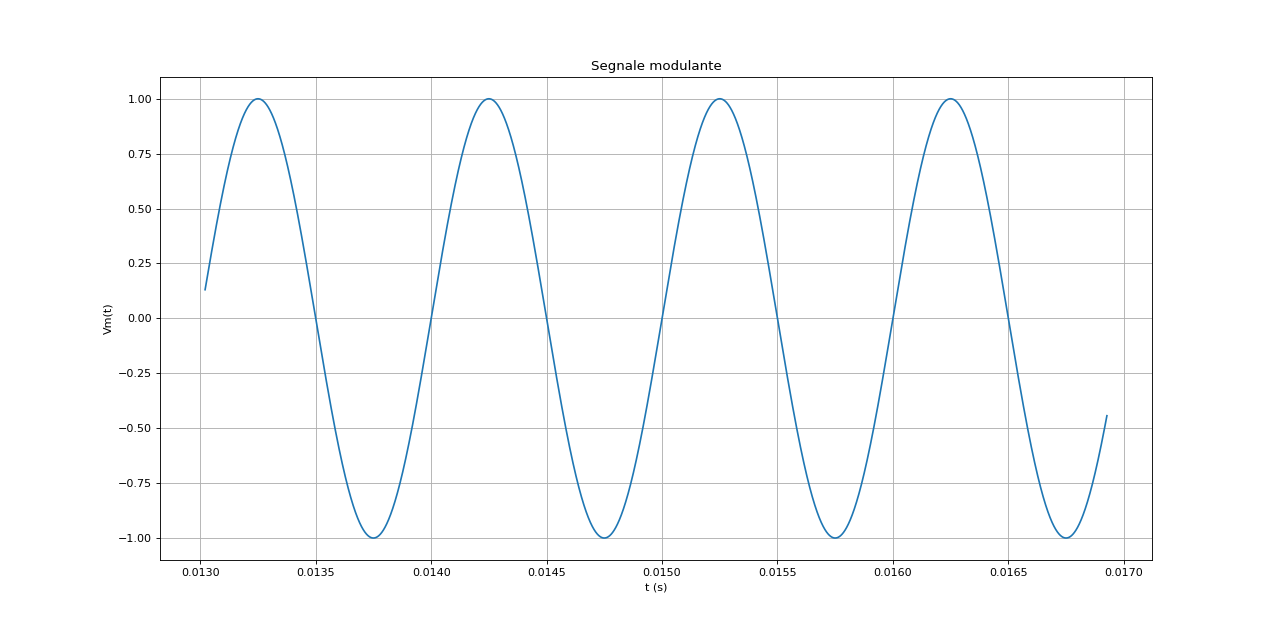
\includegraphics[width=\textwidth]{modulante.png}
\end{center}

\begin{center}
    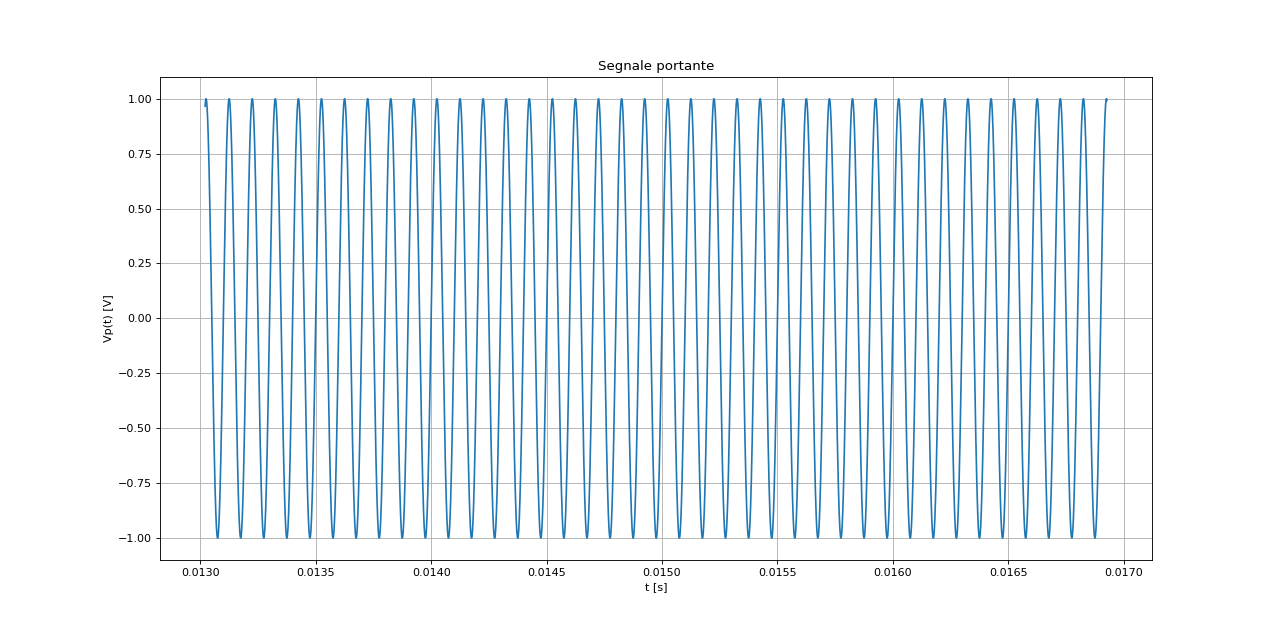
\includegraphics[width=\textwidth]{portante.png}
\end{center}

\newpage
Che uniti vengono modulati nel seguente segnale.

\begin{center}
    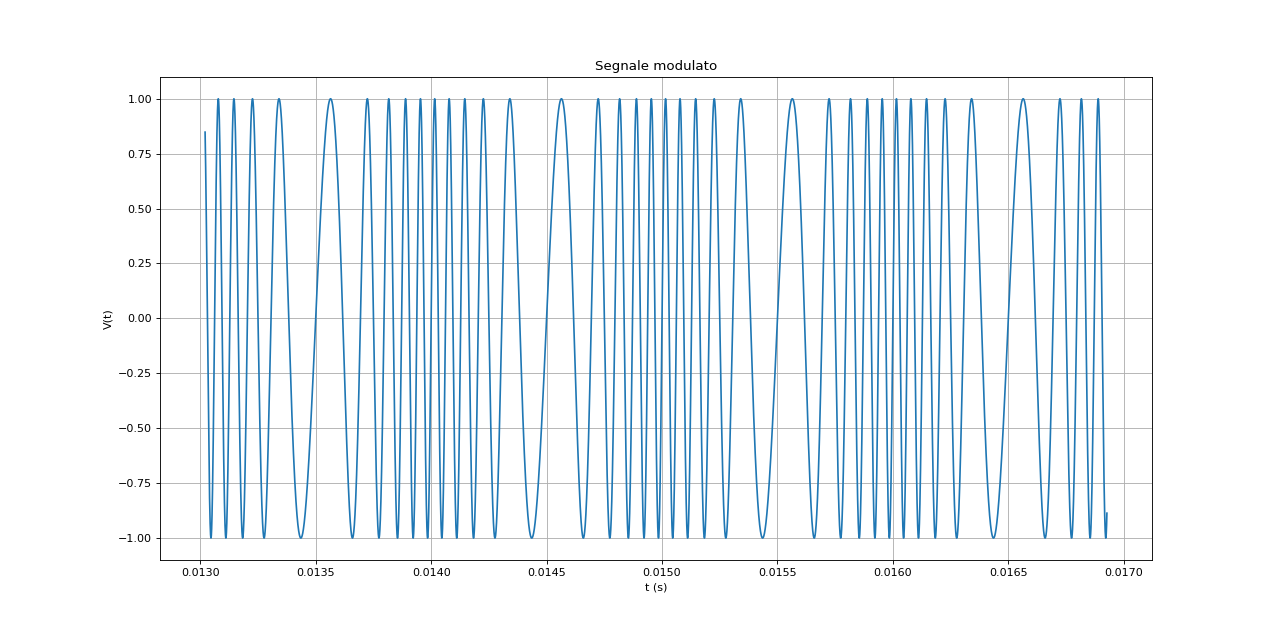
\includegraphics[width=\textwidth]{modulato.png}
\end{center}

\section{Demodulazione}
\subsection{Filtro passa basso}
Per poter tornare al segnale modulante di partenza, il primo passo è quello di applicare un filtro passa-basso.
Nel caso concreto, la frequenza di taglio del filtro è pari al 70\% della frequenza della portante, che in 
questo caso è pari a $7 kHz$.
\\
Per implementare un filtro passa basso nel software è sufficiente un ciclo for con il seguente codice:
\begin{verbatim}
def low_pass_filter(signal: List[float], tau: float) -> List[float]:
    output = np.zeros_like(signal)

    output[0] = tau * signal[0]
    for i in range(1, len(modulated)):
        output[i] = output[i - 1] + tau * (signal[i] - output[i - 1])

    return output
\end{verbatim}

\begin{center}
    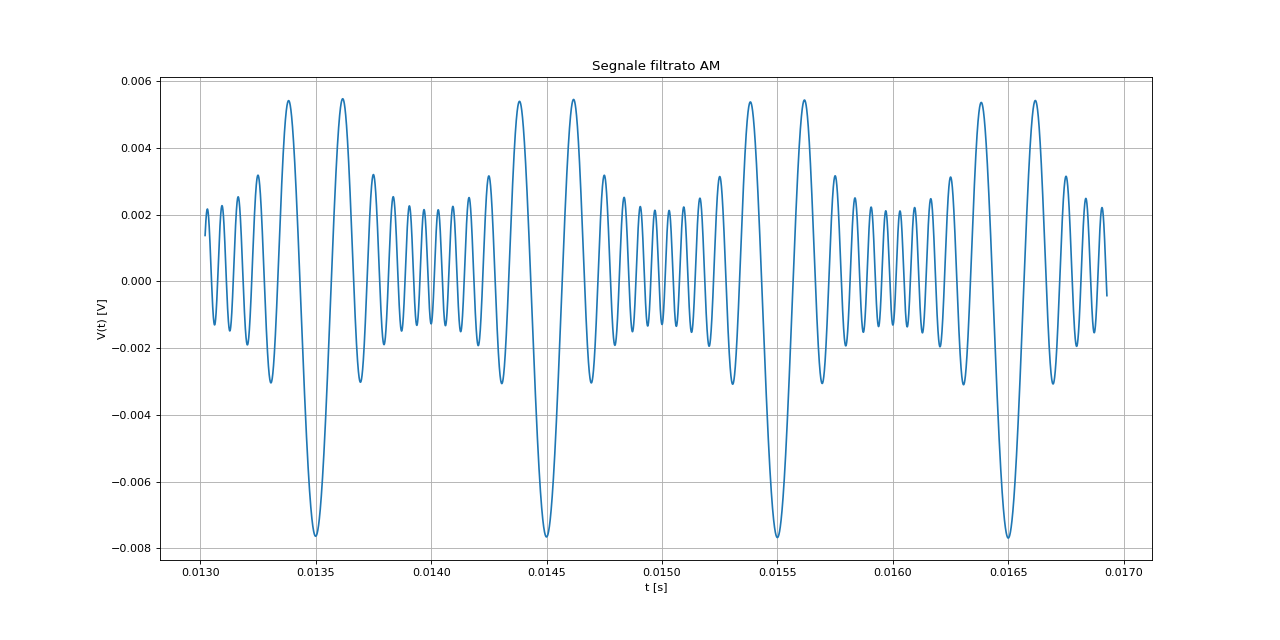
\includegraphics[width=\textwidth]{filtrato.png}
\end{center}

\end{document}
